\begin{scanpage}{0156}{138}
\begin{center}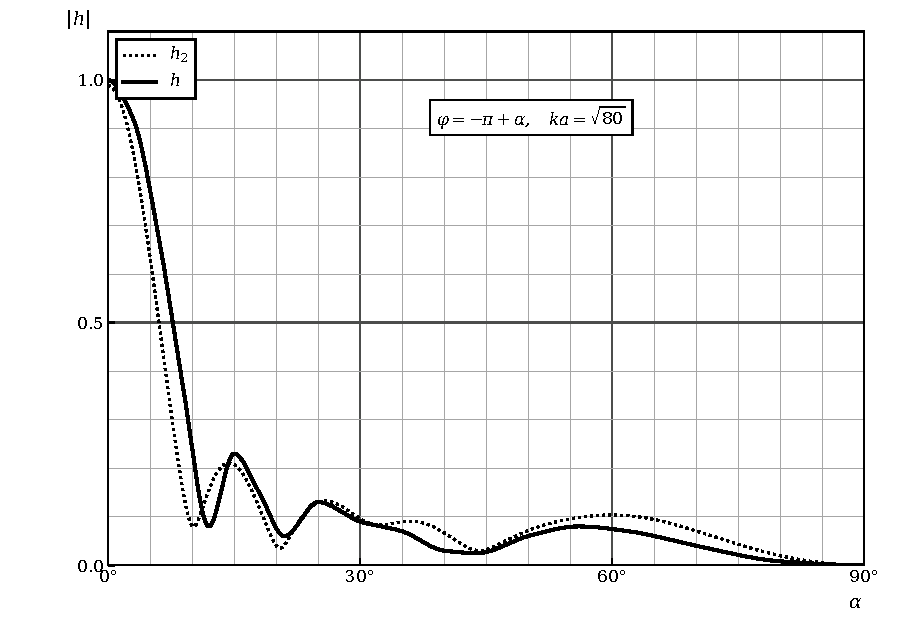
\includegraphics[width=.55\linewidth]{images/recreated/c-0156-fig54.pdf}\par
Figure 54. The same as Figure 52 when $\phi=-\pi+\alpha$.
\end{center}
Let us note that the functions $e(\alpha,\phi)$ and $h(\alpha,\phi)$ for Figures 49--52 were calculated on the basis of rigorous series which were obtained by the separation of variables in the elliptic coordinate system (compare [23])$^{(1)}$.
\sectiontitle{24}{Secondary Diffraction by a Disk}
Let us refine the approximate solution of the diffraction problem for a disk which was found in Chapter II.

Let an infinitely thin, ideally conducting disk of radius $a$ be found in free space. Let us orientate the spherical coordinate system in such a way that the normal $\mathbf n$ to the incident wave front would lie in the half-plane $\phi=\pi/2$, and form an angle $\gamma$ ($0<\gamma<\pi/2$) with the $z$ axis (Figure 63). Let us prescribe the incident plane wave field in
\[
\mathbf E=\mathbf E_0e^{ik(y\sin\gamma+z\cos\gamma)},\quad\mathbf H=\mathbf H_0e^{ik(y\sin\gamma+z\cos\gamma)}.\tag{24.01}
\]
\par\bigskip\hrule\smallskip
$(1)$Footnote appears on page 162.
\end{scanpage}
